\section{Overview}
The Internet has allowed more people than ever before in the history of the human race to be in contact with each other, and encouraged the sharing of news, commerce, education, entertainment and ideas among other things. As such, it is an extremely valuable resource, and one whose propagation should be encouraged. Internet access is now reaching the remotest parts of the globe. In particular, this means that a lot of people now have access to the World Wide Web, who have never interacted with any such technology before. Combined with the security vulnerabilities which are a product of the functional design of the Internet, this makes for a situation where a huge majority of the users of the Internet, being non tech-savvy people, can be exploited by malicious entities.

\begin{figure}
\centering
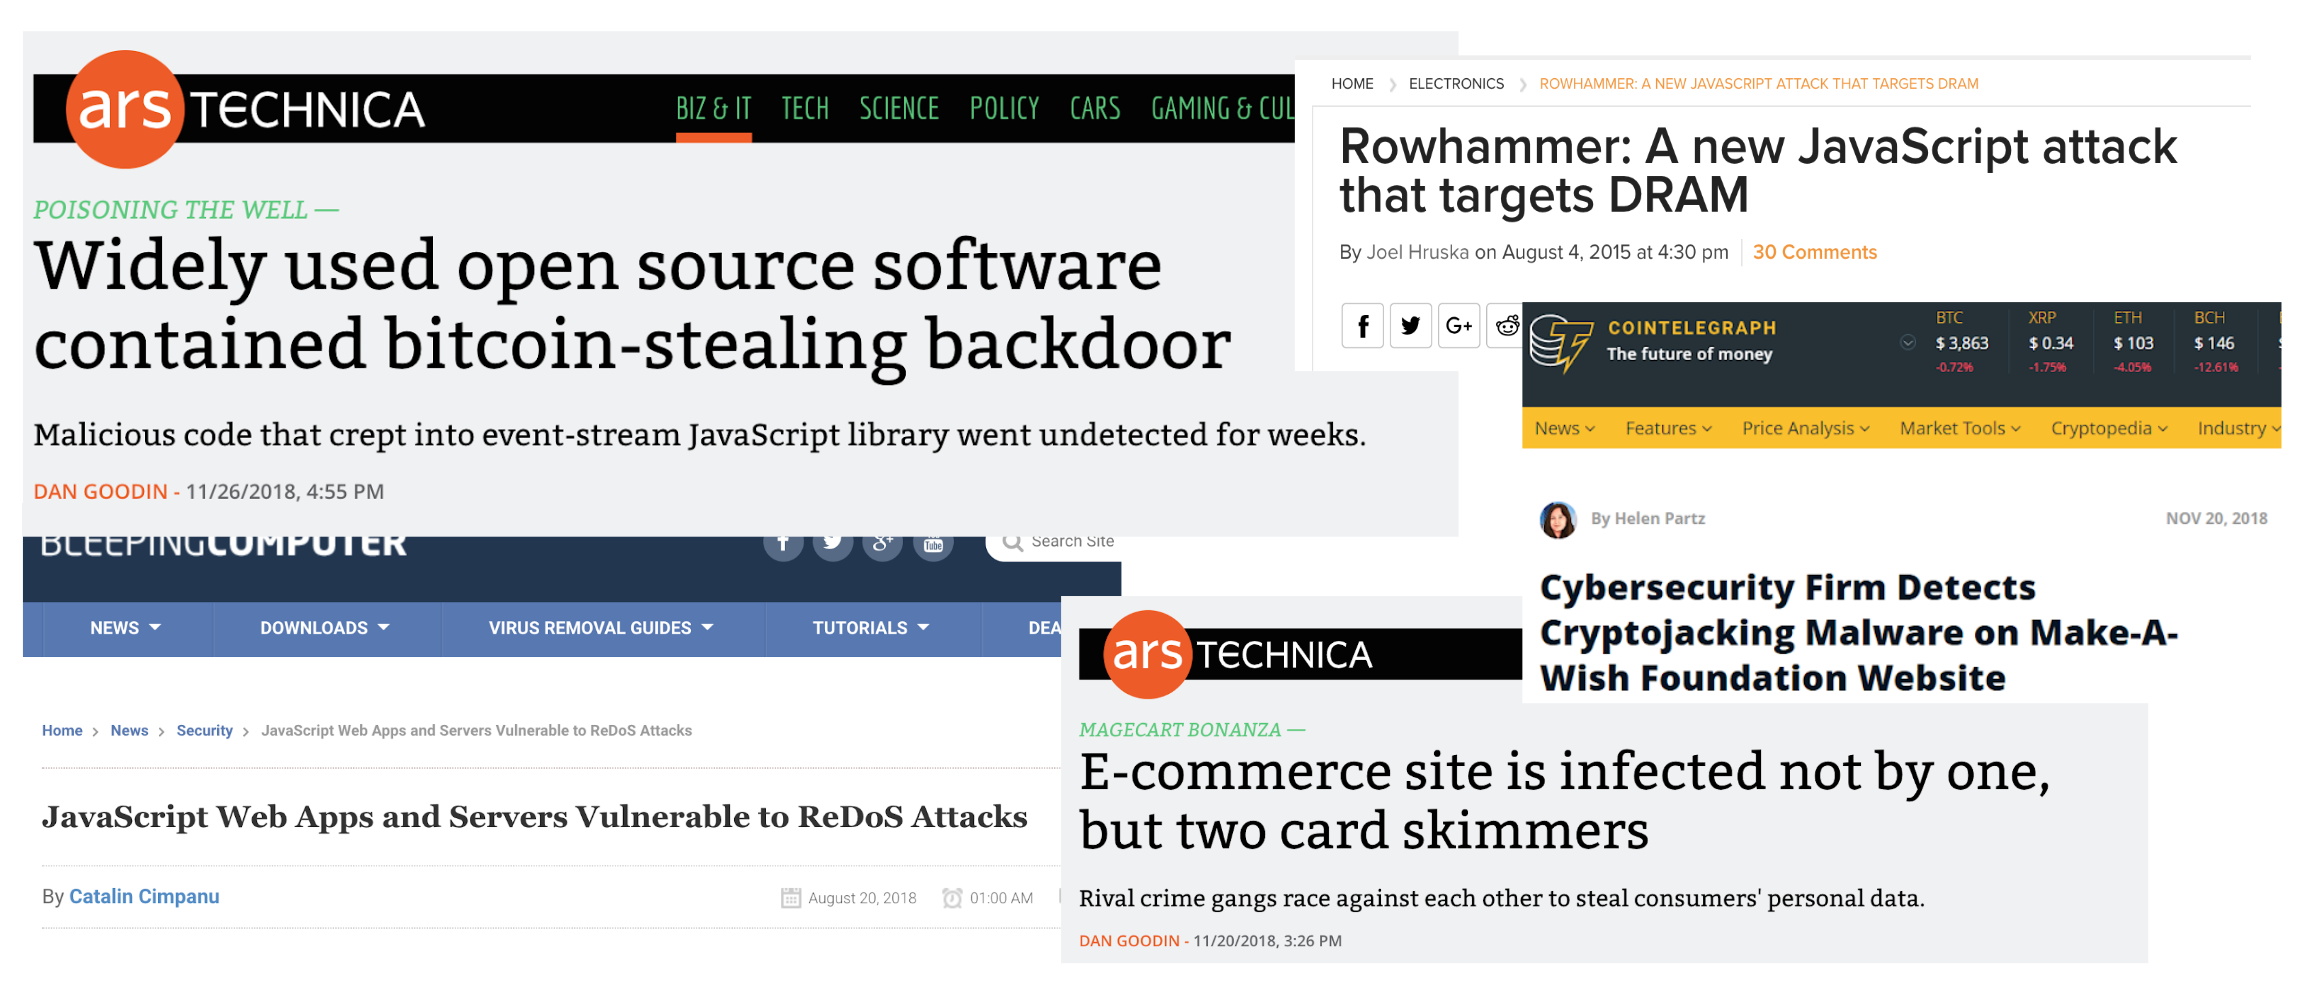
\includegraphics[width=1.0\textwidth]{images/news.png}
\caption{\label{fig:news} An example of Internet security breaches in the news}
\end{figure}

%\begin{wrapfigure}{R}{0.5\textwidth}
%\centering
%\includegraphics[width=0.4\textwidth]{trace.png}
%\caption{\label{fig:trace1} An example of a trace file}
%\end{wrapfigure}

One of the biggest dangers in using the Internet comes from the client-side (user-side) language Javascript. Javascript is a highly dynamic language that is used by 95\% of all websites on the World Wide Web. The Javascript library ecosystem is complex and unorganized. There are no reliable vulnerability databases, there are few or no details on security issues in release notes and it is often difficult to determine which versions of a library are affected by specific vulnerabilities. Security is thus an afterthought. The problem is compounded by the fact that even when vulnerabilities are fixed, a lot of websites are atrociously slow to update with the fixes. A recent work studying data from over 133k websites, showed that 37\% of them include at least one library with a known vulnerability; the time lag behind the newest release of a library is measured in the order of years\textsuperscript{\cite{LauingerCA0WK17}}. In addition, static analysis of website source code is in most cases insufficient to determine security threats.

\begin{figure}
\centering
\includegraphics[width=0.6\textwidth]{images/trace.png}
\caption{\label{fig:trace1} An example of a trace file}
\end{figure}

Thus, there is a huge a need to study and analyze what are the modes of vulnerability, and avenues of attack for malicious entities. In this project we aim to analyze Javascript ``traces'' - execution logs of all scripts executed on a website as it's loaded\textsuperscript{\ref{fig:trace1}}. The traces are stored in JSON and they contain details of every API call made by the user's browser as the page is loaded - information such as class name, function type, execution type, arguments, and return values. These traces were collected by researchers in Professor Michael Bailey's research group by crawling 939,427 websites. This represents an enormous amount of data - especially as when we started analyzing it we found out that some websites load more than 5,000 scripts, and each of these scripts can contain millions of characters. One of the biggest challenges with this project thus turned out to be just managing the huge amount of raw data. For demonstrating our methods, we decided to use the top 3k websites from Alexa, and we used a few hundred script files per website on average.

The first part of the project was data cleaning. We needed to make the data compatible with SQL. For the purposes of this project, we regard any data that contains non-ascii characters as dirty. We made this decision because cleaning the data to be ascii characters would make it easily usable with SQL as well as other readily available tools. We used the string encoder/decoder from Python 3 to process the strings and convert raw bytes into human readable text. We use regex to escape special, non-english characters and extraneous whitespace. Here we realized we couldn't process entire trace files at once - the regex processing failed at various times because of non-unicode characters. This was made especially hard because in a surprising amount of cases the entire HTML content of a website was being returned as a return value of a script. We had to spend time manually looking through the result of the initial cleaning runs and refining our regex expressions.

The second main part is flattening the nested JSON structure, and converting the data into a format that can be loaded into a SQL database. We constructed a SQL schema which is outlined in the Approach section of this report, and created a MySQL 5.7 database to house the cleaned data.
